%\documentclass[11pt, a4paper,dalthesis]{report}    % final
%\documentclass[11pt,a4paper,dalthesis]{report}
%\documentclass[11pt,a4paper,dalthesis]{book}

\documentclass[11pt,a4paper,titlepage,oneside,openany]{article}

\pagestyle{plain}
%\renewcommand{\baselinestretch}{1.7}

\usepackage{setspace}
%\singlespacing
\onehalfspacing
%\doublespacing
%\setstretch{1.1}

\usepackage{amsmath}
\usepackage{amssymb}
\usepackage{amsthm}
\usepackage{multicol}

\usepackage[margin=3cm]{geometry}
\usepackage{graphicx,psfrag}%\usepackage{hyperref}
\usepackage[small]{caption}
\usepackage{subfig}

\usepackage{algorithm}
\usepackage{algorithmic}
\newcommand{\theHalgorithm}{\arabic{algorithm}}

\usepackage{varioref} %NB: FIGURE LABELS MUST ALWAYS COME DIRECTLY AFTER CAPTION!!!
%\newcommand{\vref}{\ref}

\usepackage{index}
\makeindex
\newindex{sym}{adx}{and}{Symbol Index}
%\newcommand{\symindex}{\index[sym]}
%\newcommand{\symindex}[1]{\index[sym]{#1}\hfill}
\newcommand{\symindex}[1]{\index[sym]{#1}}

%\usepackage[breaklinks,dvips]{hyperref}%Always put after varioref, or you'll get nested section headings
%Make sure this is after index package too!
%\hypersetup{colorlinks=false,breaklinks=true}
%\hypersetup{colorlinks=false,breaklinks=true,pdfborder={0 0 0.15}}


%\usepackage{breakurl}

\graphicspath{{./images/}}

\usepackage[subfigure]{tocloft}%For table of contents
\setlength{\cftfignumwidth}{3em}

\input{longdiv}
\usepackage{wrapfig}


%\usepackage{index}
%\makeindex
%\usepackage{makeidx}

%\usepackage{lscape}
\usepackage{pdflscape}
\usepackage{multicol}

\usepackage[utf8]{inputenc}

%\usepackage{fullpage}

%Compulsory packages for the PhD in UL:
%\usepackage{UL Thesis}
\usepackage{natbib}

%\numberwithin{equation}{section}
\numberwithin{equation}{section}
\numberwithin{algorithm}{section}
\numberwithin{figure}{section}
\numberwithin{table}{section}
%\newcommand{\vec}[1]{\ensuremath{\math{#1}}}

%\linespread{1.6} %for double line spacing

\usepackage{afterpage}%fingers crossed

\newtheorem{thm}{Theorem}[section]
\newtheorem{defin}{Definition}[section]
\newtheorem{cor}[thm]{Corollary}
\newtheorem{lem}[thm]{Lemma}

%\newcommand{\dbar}{{\mkern+3mu\mathchar'26\mkern-12mu d}}
\newcommand{\dbar}{{\mkern+3mu\mathchar'26\mkern-12mud}}

\newcommand{\bbSigma}{{\mkern+8mu\mathsf{\Sigma}\mkern-9mu{\Sigma}}}
\newcommand{\thrfor}{{\Rightarrow}}

\newcommand{\mb}{\mathbb}
\newcommand{\bx}{\vec{x}}
\newcommand{\bxi}{\boldsymbol{\xi}}
\newcommand{\bdeta}{\boldsymbol{\eta}}
\newcommand{\bldeta}{\boldsymbol{\eta}}
\newcommand{\bgamma}{\boldsymbol{\gamma}}
\newcommand{\bTheta}{\boldsymbol{\Theta}}
\newcommand{\balpha}{\boldsymbol{\alpha}}
\newcommand{\bmu}{\boldsymbol{\mu}}
\newcommand{\bnu}{\boldsymbol{\nu}}
\newcommand{\bsigma}{\boldsymbol{\sigma}}
\newcommand{\bdiff}{\boldsymbol{\partial}}

\newcommand{\tomega}{\widetilde{\omega}}
\newcommand{\tbdeta}{\widetilde{\bdeta}}
\newcommand{\tbxi}{\widetilde{\bxi}}



\newcommand{\wv}{\vec{w}}

\newcommand{\ie}{i.e. }
\newcommand{\eg}{e.g. }
\newcommand{\etc}{etc}

\newcommand{\viceversa}{vice versa}
\newcommand{\FT}{\mathcal{F}}
\newcommand{\IFT}{\mathcal{F}^{-1}}
%\renewcommand{\vec}[1]{\boldsymbol{#1}}
\renewcommand{\vec}[1]{\mathbf{#1}}
\newcommand{\anged}[1]{\langle #1 \rangle}
\newcommand{\grv}[1]{\grave{#1}}
\newcommand{\asinh}{\sinh^{-1}}

\newcommand{\sgn}{\text{sgn}}
\newcommand{\morm}[1]{|\det #1 |}

\newcommand{\galpha}{\grv{\alpha}}
\newcommand{\gbeta}{\grv{\beta}}
%\newcommand{\rnlessO}{\mb{R}^n \setminus \vec{0}}
\usepackage{listings}
\usepackage{arydshln}

\interfootnotelinepenalty=10000

\newcommand{\sectionline}{%
  \nointerlineskip \vspace{\baselineskip}%
  \hspace{\fill}\rule{0.5\linewidth}{.7pt}\hspace{\fill}%
  \par\nointerlineskip \vspace{\baselineskip}
}

\renewcommand{\labelenumii}{\roman{enumii})}

\begin{document}

\begin{center}
  \textbf{Tutorial Sheet 5}
\end{center}
Sets:\begin{multicols}{2}\small
  $\quad$\\
  $\mb{R}$ - All real numbers positive and negative\\
    $\mb{R}^+$ - All positive real numbers including $0$\\
    $\mb{R}^-$ - All negative real numbers including $0$
    \columnbreak
    \\$[a,b]$ - All real numbers $x$ such that $a \le x \le b$\\
    $(a,b)$ - All real numbers $x$ such that $a < x < b$\\
    $[a,\infty)$ - All real numbers $x$ such that $a \le x$\\
    $(a,\infty)$ - All real numbers $x$ such that $a < x$
  \end{multicols}
\begin{enumerate}
\item Which of the following functions are well defined functions? If the function is not well defined, give a counterexample showing that it is not.
  \begin{multicols}{2}
    \begin{enumerate}
    \item $f: \mb{R} \to \mb{R},\quad f(x)=x^2+1$
    \item $f: \mb{R}^+ \to \mb{R}^+,\quad f(x)=x^2+1$
    \item $f: \mb{R}^+ \to [1,10],\quad f(x)=x^2+1$
    \item $f: \mb{R}^+ \to [1,\infty),\quad f(x)=x^2+1$
    \item $f: \mb{R}^+ \to \mb{R}^+,\quad f(x)=\sqrt[+]{x}$
    \item $f: \mb{R}^- \to \mb{R}^-,\quad f(x)=\sqrt[+]{x}$
    \item $f: \mb{R}^+ \to \mb{R}^-,\quad f(x)=\sqrt[+]{x}$
    \item $f: \mb{R}^+ \to \mb{R},\quad f(x)=\sqrt[+]{x}$
    \item $f: \mb{R} \to \mb{R},\quad f(x)=\frac{1}{x}$
    \item $f: \mb{R}\setminus\{0\} \to \mb{R},\quad f(x)=\frac{1}{x}$
    \item $f: \mb{R}^+\setminus\{0\} \to \mb{R},\quad f(x)=\frac{1}{x}$
    \item $f: \mb{R}^+\setminus\{0\} \to \mb{R},\quad f(x)=\frac{1}{x-1}$
    \item $f: \mb{R}^+\setminus\{1\} \to \mb{R}^+,\quad f(x)=\frac{1}{x-1}$
    \item $f: \mb{R} \to \mb{R},\quad f(x)=e^x$
    \item $f: \mb{R} \to \mb{R}^+,\quad f(x)=e^x-1$
    \item $f: \mb{R} \to \mb{R},\quad f(x)=\ln(x)$
    \item $f: \mb{R}^+\setminus \{0\} \to \mb{R}^+,\quad f(x)=\ln(x)$
    \item $f: \mb{R}^+\setminus \{0\} \to \mb{R},\quad f(x)=\ln(x)$
    \item $f: (1,\infty) \to \mb{R},\quad f(x)=\ln(x+1)$
    \end{enumerate}
  \end{multicols}

\item
  For each of the following well defined functions, say whether the function is one-to-one, onto, or invertible. In the case of invertible functions, give the inverse function. In the case of non-invertible functions, modify the domain and codomain of the functions to make them invertible and give the corressponding inverse function.
  \begin{multicols}{2}
    \begin{enumerate}
    \item $f: \mb{R} \to \mb{R},\quad f(x)=2x+4$
    \item $f: \mb{R} \to \mb{R},\quad f(x)=x$
    \item $f: \mb{R} \to \mb{R},\quad f(x)=x^2$
    \item $f: \mb{R} \to \mb{R}^+,\quad f(x)=x^2+4$
    \item $f: \mb{R}^+ \to \mb{R},\quad f(x)=\sqrt[+]{x}$
    \item $f: \mb{R}\setminus\{0\} \to \mb{R},\quad f(x)=\frac{1}{x}$
    \item $f: \mb{R} \to \mb{R},\quad f(x)=e^x$
    \item $f: \mb{R}^+ \to [1,\infty),\quad f(x)=e^x$
    \item $f: \mb{R}^+ \to \mb{R}^+,\quad f(x)=e^x+1$
    \item $f: \mb{R} \to \mb{R},\quad f(x)=\sin(x)$
    \item $f: (\text{-}\pi,\pi) \to [\text{-}1,1],\  f(x)=\sin(x)$
    \item $f: (\text{-}\frac{\pi}{2},\frac{\pi}{2}) \to [\text{-}1,1],\  f(x)=\sin(x)$
    \end{enumerate}
  \end{multicols}

\item
  Graph the well defined function $f: \mb{R} \to \mb{R}, \ f(x)=\cosh(x)$ on the interval $[-2,2]$. Based on the graph, give a suitable domain and codomain of the function to make it invertible.

\pagebreak

\item For each of the following graphs,
  \begin{enumerate}
    \item  Use the vertical line test to determine whether it is a graph of a well defined function mapping subsets of the reals to the reals.
    \item  Use the horizontal line test to determine over which domains and codomains(on the graph) the function is one-to-one, onto, or invertible.
  \end{enumerate}


  \begin{figure}[h!]
    \centering
    \subfloat[$y=ax+b$]{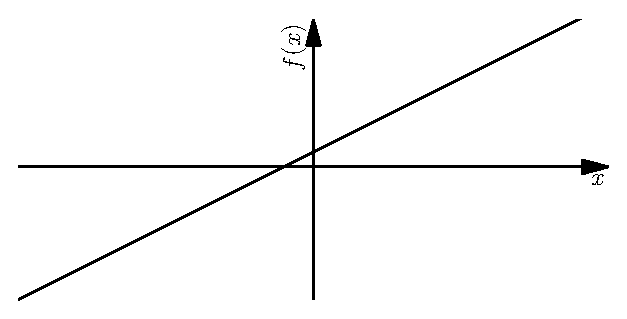
\includegraphics[width=0.45\textwidth]{functut_vht_1.eps}} \hspace{1em}
    \subfloat[$y=ax^2$]{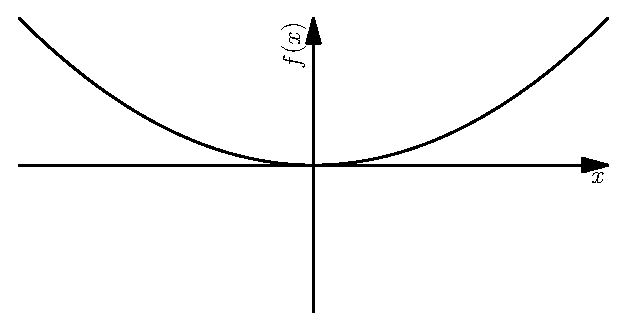
\includegraphics[width=0.45\textwidth]{functut_vht_2.eps}}\\
    \subfloat[$y^2=x$]{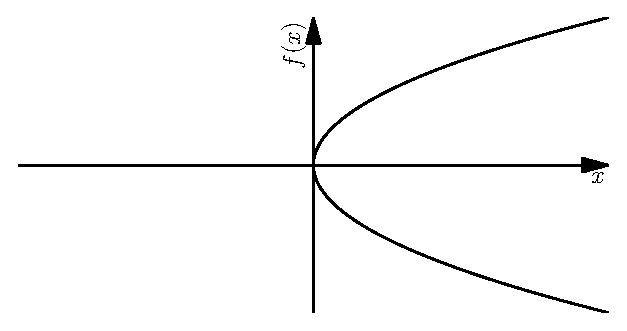
\includegraphics[width=0.45\textwidth]{functut_vht_3.eps}} \hspace{1em}
    \subfloat[$\frac{x^2}{a^2}+\frac{y^2}{b^2}=1$]{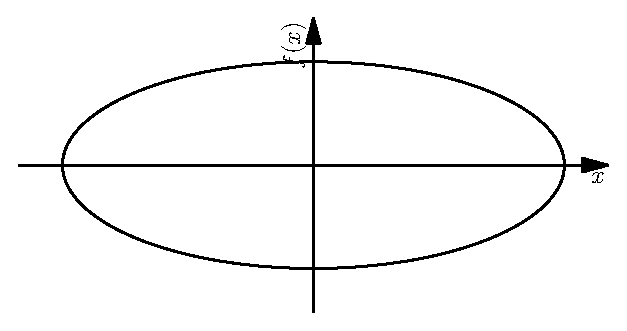
\includegraphics[width=0.45\textwidth]{functut_vht_4.eps}}\\
    \subfloat[$y=\sin(x)$]{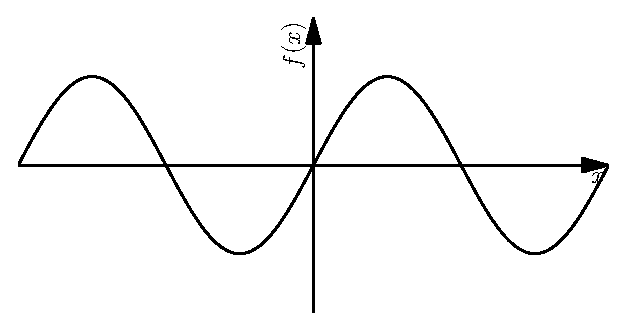
\includegraphics[width=0.45\textwidth]{functut_vht_5.eps}} \hspace{1em}
    \subfloat[$y=e^x$]{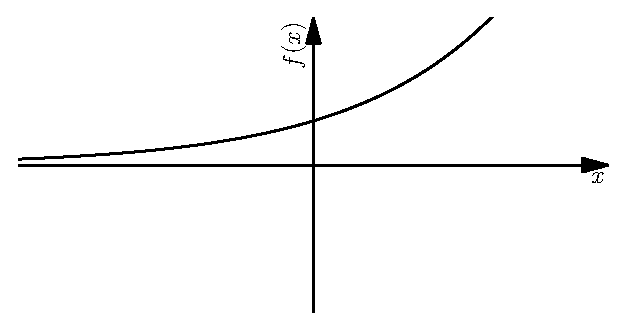
\includegraphics[width=0.45\textwidth]{functut_vht_6.eps}}\\
    \subfloat[$y=\cosh(x)$]{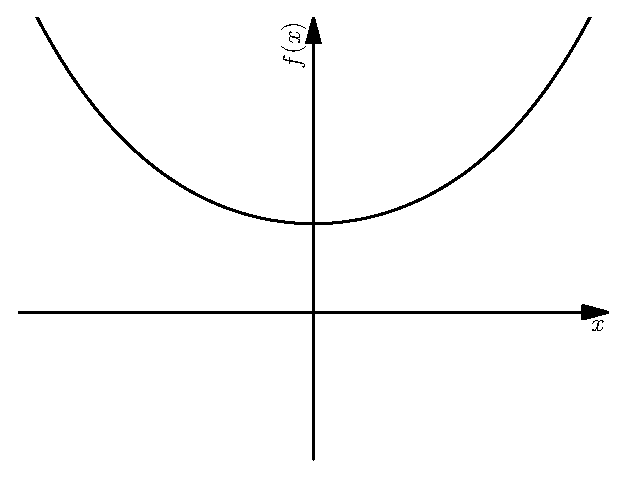
\includegraphics[width=0.4\textwidth]{functut_vht_7.eps}} \hspace{1em}
    \subfloat[$y=\sinh(x)$]{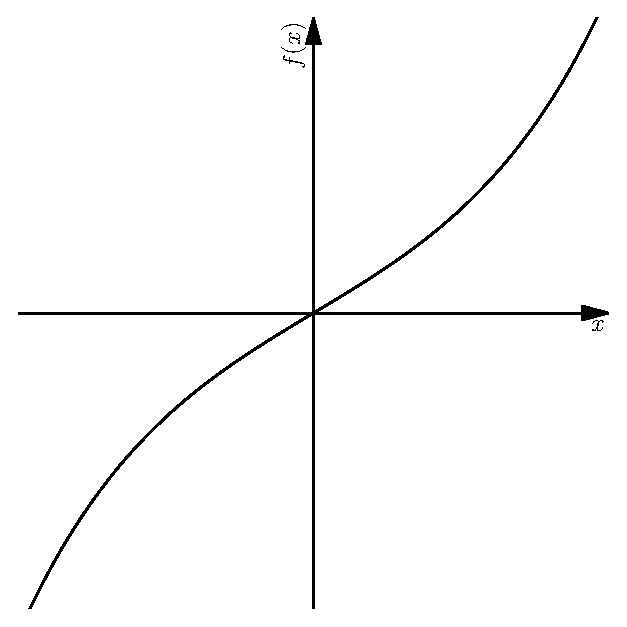
\includegraphics[width=0.4\textwidth]{functut_vht_8.eps}}\\
  \end{figure}


\end{enumerate}


\end{document}

%%% Local Variables:
%%% mode: latex
%%% TeX-master: t
%%% End:
